\documentclass[aps,prd,preprint,notitlepage,nofootinbib,superscriptaddress,floatfix]{revtex4-2}

% -------- packages --------
\usepackage{amsmath,amssymb,mathtools,bm}
\usepackage{amsthm}
\usepackage{mathrsfs}
\usepackage{booktabs}
\usepackage{array}
\usepackage{placeins}
\usepackage{xurl}
\usepackage{xcolor}
\usepackage{tikz}
\usetikzlibrary{arrows.meta,positioning,shapes.geometric,fit,calc}
\usepackage{hyperref}
\hypersetup{
  hidelinks,
  pdftitle={A Conditional Spin-c Dolbeault Index Theorem for Three Standard Model Family Copies in a Two-Center Projection Model},
  pdfauthor={Bo-Yu Chen},
  pdfsubject={Conditional Spin-c index-theoretic generation counting}
}

% -------- macros --------
\newcommand{\dd}{\mathrm{d}}
\newcommand{\ee}{\mathrm{e}}
\newcommand{\ii}{\mathrm{i}}
\newcommand{\Tr}{\operatorname{Tr}}
\newcommand{\rank}{\operatorname{rank}}
\newcommand{\Span}{\operatorname{span}}
\newcommand{\Ker}{\operatorname{Ker}}
\newcommand{\diag}{\operatorname{diag}}
\newcommand{\cB}{\mathcal B}
\newcommand{\cC}{\mathcal C}
\newcommand{\cD}{\mathcal D}
\newcommand{\cE}{\mathcal E}
\newcommand{\cH}{\mathcal H}
\newcommand{\cK}{\mathcal K}
\newcommand{\cL}{\mathcal L}
\newcommand{\cM}{\mathcal M}
\newcommand{\cO}{\mathcal O}
\newcommand{\cR}{\mathcal R}
\newcommand{\cS}{\mathcal S}
\newcommand{\CP}{\mathbb{CP}}
\newcommand{\scrD}{\mathscr D}
\newcommand{\Order}{\mathcal O}
\setlength{\emergencystretch}{2em}
\allowdisplaybreaks

\tikzset{
  psltbox/.style={draw, rounded corners=2pt, align=center, inner sep=4pt, font=\small, fill=black!3},
  psltthin/.style={draw, rounded corners=2pt, align=center, inner sep=3pt, font=\footnotesize, fill=black!2},
  psltinput/.style={draw, rounded corners=2pt, align=center, inner sep=4pt, font=\small, fill=black!8},
  psltoutput/.style={draw, rounded corners=2pt, align=center, inner sep=4pt, font=\small\bfseries, fill=black!12},
  psltarrow/.style={-{Latex[length=2mm]}, thick},
  psltdash/.style={draw, dashed, rounded corners=3pt, inner sep=6pt}
}

\newtheorem{theorem}{Theorem}
\newtheorem{proposition}{Proposition}
\newtheorem{lemma}{Lemma}
\newtheorem{corollary}{Corollary}
\theoremstyle{remark}
\newtheorem{remark}{Remark}

\begin{document}

\title{\texorpdfstring{A Conditional Spin\(^c\) Dolbeault Index Theorem for Three Standard Model Family Copies in a Two-Center Projection Model}{A Conditional Spinc Dolbeault Index Theorem for Three Standard Model Family Copies in a Two-Center Projection Model}}

\author{Bo-Yu Chen}
\affiliation{Independent Researcher}

\date{\today}

\begin{abstract}
We formulate a conditional Spin\(^c\) index-theoretic derivation of the three-family multiplicity of the Standard Model chiral representation in Projection Spectral Layer Theory (PSLT).
The input is the PSLT two-center projection datum: the compact projection surface \(C=\CP^1\), the branch divisor \(R=p_+ + p_-\), the generation line bundle \(L_R=\cO(R)\simeq\cO(2)\), and the protected SM-charged carrier \(\cR_{\rm SM}\otimes(\Lambda^{0,*}T^*C\otimes L_R)\).
On this carrier the internal fermion operator is the Spin\(^c\) Dolbeault--Dirac operator
\[
\scrD_R=\sqrt2\left(\bar\partial_{L_R}+\bar\partial_{L_R}^\dagger\right)
\]
and Hodge theory gives
\[
\Ker \scrD_R^+\cong H^0(C,L_R),
\qquad
\Ker \scrD_R^-\cong H^1(C,L_R).
\]
For \(C=\CP^1\) and \(L_R=\cO(2)\), Riemann--Roch and Serre duality give
\[
h^0(\CP^1,\cO(2))=3,
\qquad
h^1(\CP^1,\cO(2))=0.
\]
Provided all other SM-charged internal sectors are absent from the kernel or fully paired and gapped, the protected SM-charged generation sector contributes exactly three unpaired SM family copies to the four-dimensional low-energy chiral spectrum.
The novelty is not the Riemann--Roch computation itself, but the identification of the two-center projection divisor as the generation line bundle for the protected SM-charged Spin\(^c\) sector.
Scalar spectral data and the quantities \((g_N^{\rm chiral},\Gamma_N^{\rm eff},B_N)\) are kept as a post-index formation/visibility interface: they assign profiles, rates, and visible overlaps to the three protected modes, but they do not determine the family count.
\end{abstract}

\maketitle

% ============================================================
\section{Introduction and Core Structure}
\label{sec:core_structure}

The Standard Model contains three chiral copies of the same anomaly-free family representation.
This paper addresses only the multiplicity problem inside a conditional PSLT projection model: given a two-center projection surface, a generation line bundle, and a protected Spin\(^c\) carrier for SM-charged fermions, it asks whether the number of protected chiral family copies is fixed.
It does not derive the two-center projection data from a UV-complete quantum-gravity vacuum, and it does not attempt to explain Yukawa hierarchies, CKM or PMNS mixing, or the detailed mass spectrum.

Index-theoretic generation counting is a standard tool in field theory and compactification problems \cite{AtiyahSinger1968,LawsonMichelsohn1989}.
Related cohomological or topological mechanisms for chiral matter appear in heterotic, brane, and F-theory constructions \cite{Candelas1985,Witten1986,BraunHeOvrutPantev2005,BouchardDonagi2005,Blumenhagen2007,BeasleyHeckmanVafa2009}.
The specific claim here is narrower: within the PSLT protected generation sector, the two-center branch divisor \(R=p_+ + p_-\) is identified with the generation line bundle \(L_R=\cO(R)\simeq\cO(2)\), so the SM family multiplicity is the Spin\(^c\) Dolbeault index of \((\CP^1,\cO(2))\).
The novelty is therefore the physical identification of the PSLT two-center projection divisor as the generation line bundle, not the elementary Riemann--Roch calculation \(h^0(\CP^1,\cO(2))=3\) by itself.

The construction has three logically distinct layers:
\begin{enumerate}
\item the \emph{SM charge layer}, where, under the minimal one-family field-content and Yukawa assumptions, the Standard Model hypercharge pattern is fixed by gauge invariance and anomaly cancellation;
\item the \emph{internal fermion layer}, where the Spin\(^c\) Dolbeault--Dirac operator on the projection surface supplies the chiral zero-mode multiplicity;
\item the \emph{formation and visibility layer}, where the two-center conformal geometry supplies scalar spectral data for effective rates and visible-sector overlaps.
\end{enumerate}
The data needed for the Spin\(^c\) generation-multiplicity theorem are only
\begin{equation}
\boxed{
\mathfrak D_{\rm gen}
=
(C,R,L_R,\scrD_R).
}
\label{eq:generation_theorem_data}
\end{equation}
They fix \(\Ker\scrD_R^+\), hence the number of protected chiral generations.
The effective formation/visibility layer uses additional interface data
\begin{equation}
\boxed{
\mathfrak D_{\rm int}(D)
=
\left(
\pi_D,\mathfrak j_D,w_D,\mathcal J_{\rm vis}
\right).
}
\label{eq:interface_data}
\end{equation}
These interface data assign scalar profiles, rates, and visible overlaps to the protected modes; they are not inputs to the index-theoretic statement \(N_{\rm gen}=3\).
The core Hilbert-space statement is
\begin{equation}
\boxed{
\cH_{\rm chiral}^{\rm 4D}
=
\cR_{\rm SM}
\otimes
\Ker\scrD_R^+
=
\cR_{\rm SM}
\otimes
H^0(\CP^1,\cO(p_+ + p_-)).
}
\label{eq:core_hilbert}
\end{equation}
Since \(p_+ + p_-\) has degree two,
\begin{equation}
\cO(p_+ + p_-)\simeq \cO(2),
\qquad
\dim H^0(\CP^1,\cO(2))=3.
\label{eq:core_dimension}
\end{equation}
The low-energy chiral spectrum is therefore
\begin{equation}
\boxed{
\cH_{\rm chiral}^{\rm 4D}
=
\cR_{\rm SM}^{(1)}
\oplus
\cR_{\rm SM}^{(2)}
\oplus
\cR_{\rm SM}^{(3)}.
}
\label{eq:three_families}
\end{equation}
The family count is the dimension of the positive internal Spin\(^c\) fermion zero-mode space.

\begin{figure}[t]
\centering
\resizebox{\linewidth}{!}{%
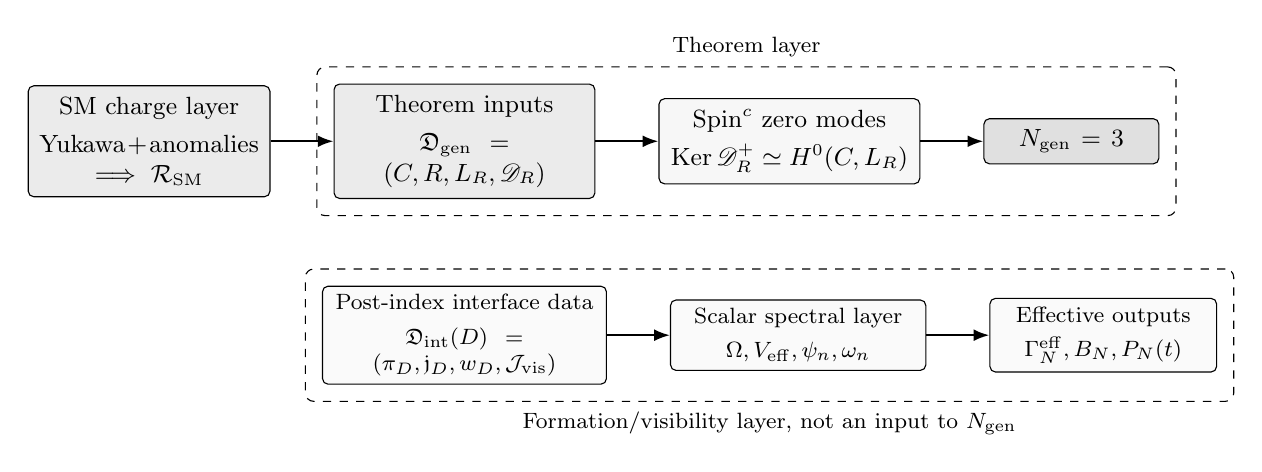
\begin{tikzpicture}[node distance=1.0cm and 0.8cm]
\node[psltinput, text width=0.23\linewidth] (charge) {SM charge layer\\[1mm]\(\text{Yukawa}+\text{anomalies}\)\\\(\Longrightarrow \cR_{\rm SM}\)};
\node[psltinput, text width=0.25\linewidth, right=of charge] (geninput) {Theorem inputs\\[1mm]\(\mathfrak D_{\rm gen}=(C,R,L_R,\scrD_R)\)};
\node[psltbox, text width=0.25\linewidth, right=of geninput] (hodge) {Spin\(^c\) zero modes\\[1mm]\(\Ker\scrD_R^+\simeq H^0(C,L_R)\)};
\node[psltoutput, text width=0.16\linewidth, right=of hodge] (ngen) {\(N_{\rm gen}=3\)};
\draw[psltarrow] (charge) -- (geninput);
\draw[psltarrow] (geninput) -- (hodge);
\draw[psltarrow] (hodge) -- (ngen);

\node[psltthin, text width=0.28\linewidth, below=1.1cm of geninput] (interface) {Post-index interface data\\[1mm]\(\mathfrak D_{\rm int}(D)=(\pi_D,\mathfrak j_D,w_D,\mathcal J_{\rm vis})\)};
\node[psltthin, text width=0.25\linewidth, right=of interface] (scalar) {Scalar spectral layer\\[1mm]\(\Omega,V_{\rm eff},\psi_n,\omega_n\)};
\node[psltthin, text width=0.22\linewidth, right=of scalar] (rates) {Effective outputs\\[1mm]\(\Gamma_N^{\rm eff},B_N,P_N(t)\)};
\draw[psltarrow] (interface) -- (scalar);
\draw[psltarrow] (scalar) -- (rates);

\node[psltdash, fit=(geninput)(hodge)(ngen), label={[font=\footnotesize]above:Theorem layer}] {};
\node[psltdash, fit=(interface)(scalar)(rates), label={[font=\footnotesize]below:Formation/visibility layer, not an input to \(N_{\rm gen}\)}] {};
\end{tikzpicture}
}
\caption{Logical architecture of the PSLT Spin\(^c\) generation theorem.
The Standard Model charge layer fixes one anomaly-free chiral family representation \(\cR_{\rm SM}\).
The protected internal fermion layer uses the two-center projection data \(C=\CP^1\), \(R=p_+ + p_-\), \(L_R=\cO(R)\simeq\cO(2)\), and the Spin\(^c\) Dolbeault--Dirac operator \(\scrD_R\) to prove the family multiplicity through \(\Ker\scrD_R^+\simeq H^0(C,L_R)\).
The scalar spectral, kinetic, and visibility data form a post-index effective interface and are not inputs to the theorem \(N_{\rm gen}=3\).}
\label{fig:logical_architecture}
\end{figure}

\begin{table}[t]
\caption{Assumption boundary and theorem scope.
The theorem proves the three-family multiplicity inside the protected PSLT Spin\(^c\) generation sector.
Effective scalar spectral quantities and formation/visibility weights are post-index interface data and are not used to prove \(N_{\rm gen}=3\).}
\label{tab:assumption_boundary}
\centering
\small
\newcommand{\tblcell}[2]{\parbox[t]{#1}{#2}}
\begin{tabular}{@{}lll@{}}
\toprule
\tblcell{1.75in}{Object or claim} & \tblcell{1.85in}{Status in this paper} & \tblcell{2.15in}{Role} \\
\midrule
\tblcell{1.75in}{\(C=\CP^1\)} & \tblcell{1.85in}{PSLT two-center projection datum} & \tblcell{2.15in}{Input} \\
\tblcell{1.75in}{\(R=p_+ + p_-\)} & \tblcell{1.85in}{PSLT branch divisor} & \tblcell{2.15in}{Input} \\
\tblcell{1.75in}{\(L_R=\cO(R)\simeq\cO(2)\)} & \tblcell{1.85in}{Determined by \(R\) on \(\CP^1\)} & \tblcell{2.15in}{Generation line bundle} \\
\tblcell{1.75in}{\(\Lambda^{0,*}T^*C\otimes L_R\)} & \tblcell{1.85in}{Assumed protected carrier} & \tblcell{2.15in}{Spin\(^c\) internal fermion sector} \\
\tblcell{1.75in}{\(\scrD_R\)} & \tblcell{1.85in}{Specified Spin\(^c\) Dolbeault--Dirac operator} & \tblcell{2.15in}{Counts protected zero modes} \\
\tblcell{1.75in}{\(h^0=3,\ h^1=0\)} & \tblcell{1.85in}{Theorem consequence} & \tblcell{2.15in}{Three protected chiral copies} \\
\tblcell{1.75in}{Vectorlike gap for other SM-charged sectors} & \tblcell{1.85in}{Assumption} & \tblcell{2.15in}{Excludes extra light SM-charged exotics} \\
\tblcell{1.75in}{\(\Omega,V_{\rm eff},\Gamma_N^{\rm eff},B_N,P_N\)} & \tblcell{1.85in}{Effective post-index interface} & \tblcell{2.15in}{Formation/visibility, not family-count proof} \\
\tblcell{1.75in}{UV derivation of \((C,R,L_R)\)} & \tblcell{1.85in}{Not proven here} & \tblcell{2.15in}{Future strengthening} \\
\bottomrule
\end{tabular}
\end{table}

\subsection{Notation conventions}
\label{sec:notation_conventions}

Throughout the paper, \(D\) denotes the two-center separation parameter.
Dirac-type operators are written with script letters, such as \(\scrD_R\), \(\scrD_X\), \(\scrD_{\rm vec}\), and \(\scrD_{M_4}^{\rm SM}\).
The Bergman projector onto \(H^0(C,L_R)\) is \(P_R\), the collective-coordinate projector is \(P_N^{\rm cc}\), the one-dimensional Toeplitz-mode projector is \(\Pi_N=|u_N\rangle\langle u_N|\), and the observed layer probability is \(P_N(t;D,\eta)\).
The protected zero-mode degeneracy is denoted \(g_N^{\rm chiral}\); any unadorned degeneracy symbol is avoided in the chiral family count.

% ============================================================
\section{Two-Center Projection Data and Topological Constraint}
\label{sec:parent_data}

Let \(M_4\) be four-dimensional spacetime and let the compact projection surface be
\begin{equation}
C\simeq\CP^1.
\end{equation}
The two projection branch points define the divisor
\begin{equation}
R=p_+ + p_-,
\qquad
L_R=\cO(R)\simeq\cO(2).
\label{eq:LR_def}
\end{equation}
For bookkeeping we denote a possible effective decomposition by
\begin{equation}
S_{\rm eff}
=
S_{\rm grav}
+S_{\rm gauge}
+S_{\rm Higgs}
+S_{\rm fermion}
+S_\Omega^{\rm cov}
+S_{\rm proj}
+S_{\rm vis}.
\label{eq:parent_action}
\end{equation}
No UV-complete parent action is derived in this paper.
The theorem uses only the projection data and the cohomological constraint below.
The projection sector fixes the topological class of \(L_R\), not a pointwise equality between a smooth curvature form and a delta-current.
The robust condition is the cohomological constraint
\begin{equation}
\boxed{
\left[\frac{\ii}{2\pi}F_{A_R}\right]
=
\operatorname{PD}(R)
=
[p_+]+[p_-]
\in H^2(C,\mathbb Z),
\qquad
R=p_+ + p_-.
}
\label{eq:Sproj_cohomology}
\end{equation}
Equivalently,
\begin{equation}
c_1(L_R)=\operatorname{PD}(R),
\qquad
\deg L_R=2.
\label{eq:degree_LR}
\end{equation}
When an action-like expression is useful, it should be read as a topological constraint or as a regulated current limit:
\begin{equation}
S_{\rm proj}^{\rm top}
=
\int_C\lambda_R
\left[
\frac{\ii}{2\pi}F_{A_R}
-J_R^{(\varepsilon)}
\right],
\label{eq:Sproj}
\end{equation}
where \(J_R^{(\varepsilon)}\) is any smooth representative of \(\operatorname{PD}(R)\) that tends, as a current, to \(\delta_{p_+}^{(2)}+\delta_{p_-}^{(2)}\).
The topological input is Eq.~\eqref{eq:Sproj_cohomology}; Eq.~\eqref{eq:Sproj} is only a regulated implementation of the same cohomology class.

\begin{figure}[t]
\centering
\resizebox{\linewidth}{!}{%
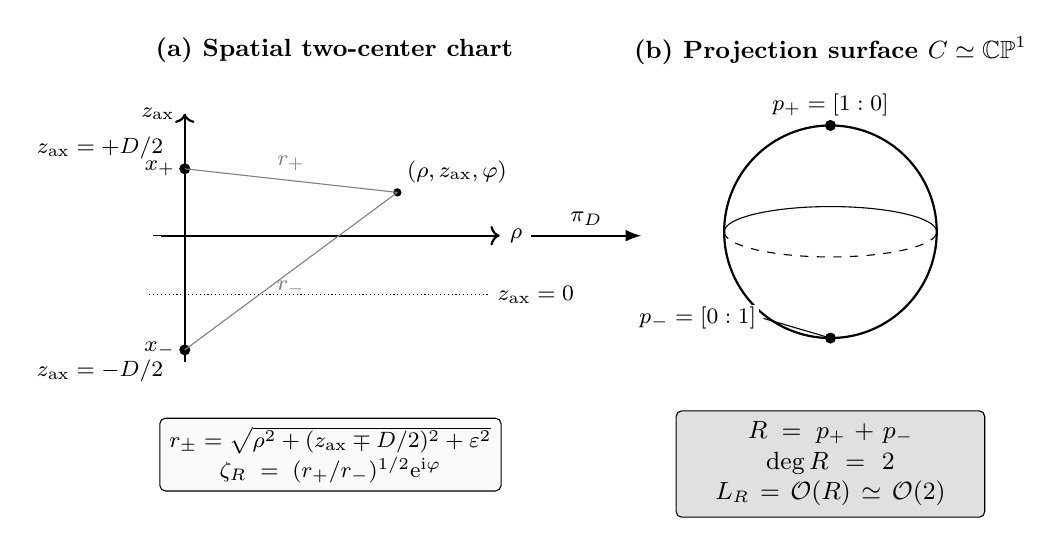
\begin{tikzpicture}[scale=1.0, every node/.style={font=\footnotesize}]
% spatial panel
\node[font=\small\bfseries] at (-3.2,2.35) {(a) Spatial two-center chart};
\draw[->, thick] (-5.1,-1.6) -- (-5.1,1.55) node[left] {\(z_{\rm ax}\)};
\draw[->, thick] (-5.4,0) -- (-1.1,0) node[right] {\(\rho\)};
\draw[dashed] (-5.5,0) -- (-1.2,0);
\draw[densely dotted] (-5.55,-0.75) -- (-1.25,-0.75) node[right] {\(z_{\rm ax}=0\)};
\fill (-5.1,0.85) circle (2pt) node[left] {\(x_+\)};
\fill (-5.1,-1.45) circle (2pt) node[left] {\(x_-\)};
\node[above left] at (-5.25,0.85) {\(z_{\rm ax}=+D/2\)};
\node[below left] at (-5.25,-1.45) {\(z_{\rm ax}=-D/2\)};
\coordinate (probe) at (-2.4,0.55);
\fill (probe) circle (1.5pt) node[above right] {\((\rho,z_{\rm ax},\varphi)\)};
\draw[gray] (-5.1,0.85) -- (probe) node[midway, above] {\(r_+\)};
\draw[gray] (-5.1,-1.45) -- (probe) node[midway, below] {\(r_-\)};
\node[psltthin, text width=0.34\linewidth] at (-3.25,-2.78)
{\(r_\pm=\sqrt{\rho^2+(z_{\rm ax}\mp D/2)^2+\varepsilon^2}\)\\
\(\zeta_R=(r_+/r_-)^{1/2}\ee^{\ii\varphi}\)};

% arrow
\draw[psltarrow] (-0.7,0.0) -- (0.7,0.0) node[midway, above] {\(\pi_D\)};

% CP1 panel
\node[font=\small\bfseries] at (3.1,2.35) {(b) Projection surface \(C\simeq\CP^1\)};
\draw[thick] (3.1,0.05) circle (1.35);
\draw[dashed] (1.75,0.05) arc[start angle=180,end angle=360,x radius=1.35,y radius=0.32];
\draw (1.75,0.05) arc[start angle=180,end angle=0,x radius=1.35,y radius=0.32];
\fill (3.1,1.4) circle (2pt) node[above] {\(p_+=[1:0]\)};
\coordinate (pminusfig) at (3.1,-1.3);
\fill (pminusfig) circle (2pt);
\draw[thin] (pminusfig) -- (2.25,-1.05);
\node[anchor=east, fill=white, inner sep=1pt] at (2.20,-1.05) {\(p_-=[0:1]\)};
\node[psltoutput, text width=0.30\linewidth] at (3.1,-2.90)
{\(R=p_+ + p_-\)\\
\(\deg R=2\)\\
\(L_R=\cO(R)\simeq\cO(2)\)};
\end{tikzpicture}
}
\caption{Two-center projection geometry and the generation divisor.
The spatial chart contains two ordered centers \(x_\pm\) at \(z_{\rm ax}=\pm D/2\), with regulated distances \(r_\pm\).
The projection map \(\pi_D\) sends the regulated two-center chart to \(C\simeq\CP^1\), and in the collapsed-core limit maps the centers to the branch points \(p_+\) and \(p_-\).
The divisor \(R=p_+ + p_-\) has degree two and defines the generation line bundle \(L_R=\cO(R)\simeq\cO(2)\).
The midplane normalization \(z_{\rm ax}=0\Rightarrow |\zeta_R|=1\) fixes the residual scale of the affine coordinate.}
\label{fig:two_center_projection}
\end{figure}

\subsection{SM-charged fermion sector}
\label{sec:sm_fermion_sector}

The SM-charged internal fermion carrier is assumed to be exactly
\begin{equation}
\cE_{\rm gen}
=
\cR_{\rm SM}\otimes \cS_C,
\qquad
\cS_C=\Lambda^{0,*}T^*C\otimes L_R.
\label{eq:generation_carrier}
\end{equation}

Let
\begin{equation}
X=M_4\times C.
\end{equation}
The generation-sector product Dirac operator is
\begin{equation}
\boxed{
\scrD_X
=
\scrD_{M_4}^{\rm SM}\otimes 1
+
\gamma_5\otimes\scrD_R,
\qquad
\Gamma_X=\gamma_5\otimes\Gamma_C.
}
\label{eq:product_dirac}
\end{equation}
Here \(\scrD_{M_4}^{\rm SM}\) includes the four-dimensional SM gauge connection on \(\cR_{\rm SM}\), \(\Gamma_C\) is the internal Spin\(^c\) chirality, and \(\Gamma_X\) is the product chirality.
The generation-sector fermion action is
\begin{equation}
\boxed{
S_{\rm fermion}^{\rm gen}
=
\int_{M_4\times C}
\dd{\rm vol}_{M_4}\,\dd{\rm vol}_{C}\,
\overline{\Psi}\,\ii\scrD_X\Psi .
}
\label{eq:product_fermion_action}
\end{equation}
The internal mode expansion is
\begin{equation}
\Psi(x,y)
=
\sum_{\alpha}\psi_\alpha^+(x)u_\alpha^+(y)
+
\sum_{\beta}\psi_\beta^-(x)u_\beta^-(y)
+
\sum_{\lambda>0}\Psi_\lambda(x)\chi_\lambda(y),
\label{eq:product_mode_expansion}
\end{equation}
where
\begin{equation}
\scrD_Ru_\alpha^+=0,
\qquad
u_\alpha^+\in\Ker\scrD_R^+,
\qquad
\scrD_Ru_\beta^-=0,
\qquad
u_\beta^-\in\Ker\scrD_R^-.
\label{eq:internal_zero_mode_conditions}
\end{equation}
After a fixed product-chirality projection, internal positive and negative zero modes produce opposite four-dimensional Weyl chiralities.
We choose the product chirality so that \(\Ker\scrD_R^+\) carries the left-handed SM family representation \(\cR_{\rm SM}\); \(\Ker\scrD_R^-\) would supply the opposite four-dimensional chirality in the same generation sector.
Thus the chain is explicit:
\begin{equation}
\begin{gathered}
\text{internal Spin}^{c}\text{ zero mode}
\quad\Longrightarrow\quad
\text{massless 4D Weyl fermion}
\\
\Longrightarrow\quad
\text{SM chiral generation}.
\end{gathered}
\end{equation}

All other SM-charged internal sectors are required to be vectorlike and genuinely gapped:
\begin{equation}
\cE_{\rm fermion}^{\rm SM}
=
\cE_{\rm gen}
\oplus
\cE_{\rm vec}.
\label{eq:exclusivity_vec}
\end{equation}
The condition is stronger than \(\operatorname{ind}\scrD_{\rm vec}=0\).
It requires either
\begin{equation}
\Ker\scrD_{\rm vec}=0,
\label{eq:vec_no_kernel}
\end{equation}
or
\begin{equation}
\begin{aligned}
\dim\Ker\scrD_{\rm vec}^+
\;&=
\dim\Ker\scrD_{\rm vec}^-,
\\
M_{\rm vec}:\Ker\scrD_{\rm vec}^+
\;&\longrightarrow
\Ker\scrD_{\rm vec}^-,
\qquad
M_{\rm vec}\text{ is full rank and gauge invariant}.
\end{aligned}
\label{eq:vectorlike_gap_condition}
\end{equation}
Index zero only excludes extra net chirality.
Equation~\eqref{eq:vec_no_kernel} or Eq.~\eqref{eq:vectorlike_gap_condition} is the additional low-energy condition that excludes unpaired massless SM-charged vectorlike exotics.
SM-neutral sectors may be present, but they do not carry generation quantum numbers:
\begin{equation}
\cE_{\rm fermion}
=
\cE_{\rm gen}
\oplus
\cE_{\rm vec}
\oplus
\cE_{\rm neutral}.
\label{eq:fermion_sector_decomp}
\end{equation}
This is the exclusivity condition needed for the conditional no-fourth-family statement within the protected SM-charged sector.
Without it, the Spin\(^c\) theorem proves only the three-dimensionality of the protected generation sector, not the absence of additional SM-charged chiral sectors.

% ============================================================
\section{One Standard Model Family}
\label{sec:one_family}

The local anomaly equations use the Standard Model Lie algebra, with standard anomaly conventions \cite{Bertlmann1996,Bilal2008}.
When a global group and charge lattice are needed, we take
\begin{equation}
G_{\rm SM}
=
\frac{SU(3)_c\times SU(2)_L\times U(1)_Y}{\mathbb Z_6}.
\label{eq:gsm_global}
\end{equation}
This global choice fixes the conventional hypercharge unit used below; without it, the local equations determine hypercharge only up to an overall \(U(1)_Y\) normalization.
For one left-handed Weyl family, take
\begin{equation}
Q:(3,2)_{Y_Q},\quad
u^c:(\bar3,1)_{Y_u},\quad
d^c:(\bar3,1)_{Y_d},
\qquad
L:(1,2)_{Y_L},\quad
e^c:(1,1)_{Y_e},
\end{equation}
with Higgs
\begin{equation}
H:(1,2)_h.
\end{equation}
Set \(Y_Q=q\).
Gauge invariance of the Yukawa couplings gives
\begin{align}
QHu^c:&\qquad q+h+Y_u=0,
&
QH^\dagger d^c:&\qquad q-h+Y_d=0,
\\
LH^\dagger e^c:&\qquad Y_L-h+Y_e=0.
\end{align}
Hence
\begin{equation}
Y_u=-q-h,\qquad
Y_d=-q+h,\qquad
Y_e=h-Y_L.
\label{eq:yukawa_hypercharge_constraints}
\end{equation}
The \(SU(3)^2U(1)\) anomaly gives
\begin{equation}
2Y_Q+Y_u+Y_d=0,
\end{equation}
which is automatic after Eq.~\eqref{eq:yukawa_hypercharge_constraints}.
The pure color anomaly also cancels:
\begin{equation}
\mathcal A_{SU(3)^3}
=
2A(3)+A(\bar3)+A(\bar3)
=
2A(3)-A(3)-A(3)
=0,
\label{eq:su3_cubic_anomaly}
\end{equation}
where the factor of two comes from the two \(SU(2)_L\) components of \(Q\), and \(A(\bar3)=-A(3)\).
The \(SU(2)^2U(1)\) anomaly gives
\begin{equation}
3Y_Q+Y_L=0,
\qquad
Y_L=-3q.
\label{eq:su2_anomaly}
\end{equation}
The mixed gravitational anomaly requires
\begin{equation}
6Y_Q+3Y_u+3Y_d+2Y_L+Y_e=0.
\label{eq:grav_anomaly}
\end{equation}
Substitution gives
\begin{equation}
6q+3(-q-h)+3(-q+h)+2(-3q)+(h+3q)=0,
\end{equation}
so
\begin{equation}
h=3q.
\end{equation}
Therefore
\begin{equation}
Y_u=-4q,\qquad
Y_d=2q,\qquad
Y_L=-3q,\qquad
Y_e=6q,\qquad
Y_H=3q.
\end{equation}
The \(U(1)^3\) anomaly cancels:
\begin{equation}
6q^3+3(-4q)^3+3(2q)^3+2(-3q)^3+(6q)^3
=0.
\end{equation}
There is no Witten global \(SU(2)\) anomaly \cite{Witten1982SU2}.
One family contains
\begin{equation}
3\text{ color copies of }Q
+
1\text{ lepton doublet}
=4
\label{eq:witten_su2_count}
\end{equation}
left-handed \(SU(2)_L\) Weyl doublets, which is even.
For three families the number is \(12\), still even.
With \(q=1/6\),
\begin{equation}
\boxed{
(Y_Q,Y_u,Y_d,Y_L,Y_e,Y_H)
=
\left(
\frac16,
-\frac23,
\frac13,
-\frac12,
1,
\frac12
\right).
}
\label{eq:SM_hypercharges}
\end{equation}
A sterile \(\nu^c:(1,1)_0\) may be added without changing these anomaly equations.

\begin{proposition}
Within the minimal one-family chiral field content above, and assuming the Yukawa couplings \(QHu^c\), \(QH^\dagger d^c\), and \(LH^\dagger e^c\), the local anomaly equations fix the hypercharge pattern up to the overall normalization of \(U(1)_Y\).
The choice in Eq.~\eqref{eq:gsm_global} fixes the conventional unit \(q=1/6\).
\end{proposition}
This proposition fixes the one-family representation that is later tensored with the Spin\(^c\) zero-mode space; it does not determine the number of families.

% ============================================================
\section{\texorpdfstring{Spin\(^c\) Dolbeault--Dirac Zero Modes}{Spinc Dolbeault-Dirac Zero Modes}}
\label{sec:spinc_dirac}

The internal fermion operator is not the ordinary spin Dirac operator.
It is the Spin\(^c\) Dolbeault--Dirac operator
\begin{equation}
\boxed{
\scrD_R
=
\sqrt2
\left(
\bar\partial_{L_R}
+\bar\partial_{L_R}^\dagger
\right)
}
\label{eq:Dolbeault_Dirac}
\end{equation}
acting on
\begin{equation}
\cS_C
=
\Lambda^{0,*}T^*C\otimes L_R.
\label{eq:spinc_spinor_bundle}
\end{equation}
\begin{remark}[BPS-compatible origin of the Dolbeault representative]
In a BPS or worldline-supersymmetric realization of this protected generation sector, massless states are represented by \(Q\)-cohomology classes, with
\begin{equation}
Q^2=0,
\qquad
H=\{Q,Q^\dagger\}.
\end{equation}
For the holomorphic carrier
\begin{equation}
\cH_{\rm int}=\Omega^{0,*}(C,L_R),
\end{equation}
locality, first-order gauge covariance, and compatibility with the complex structure select a Cauchy--Riemann type representative
\begin{equation}
Q=\bar\partial_{L_R}
\end{equation}
up to holomorphic bundle isomorphism and gauge choice.
The corresponding Hermitian Dirac representative is therefore
\begin{equation}
\scrD_R=\sqrt2(Q+Q^\dagger)
=
\sqrt2(\bar\partial_{L_R}+\bar\partial_{L_R}^{\dagger}).
\end{equation}
This remark is only a BPS-compatible motivation for the protected PSLT sector used below; the theorem remains conditional on the two-center projection data, the holomorphic carrier \(\Omega^{0,*}(C,L_R)\), and the absence of additional flux, superpotential, Ext-complex, or torsion deformations that would replace the Dolbeault differential by a different protected complex.
It is not an unconditional vacuum-selection theorem for all string or quantum-gravity compactifications.
\end{remark}
We use the canonical Spin\(^c\) structure on the complex curve \(C\), whose untwisted spinor bundle is \(\Lambda^{0,*}T^*C\).
The line bundle \(L_R\) is an auxiliary twisting bundle for the Dolbeault--Dirac operator, not the Spin\(^c\) determinant line itself.
The relevant index is therefore the Dolbeault index
\begin{equation}
\operatorname{ind}\scrD_R
=
\chi(C,L_R)
=
h^0(C,L_R)-h^1(C,L_R).
\label{eq:dolbeault_index}
\end{equation}
Its internal chirality decomposition is
\begin{equation}
\cS_C^+
=
\Lambda^{0,0}T^*C\otimes L_R,
\qquad
\cS_C^-
=
\Lambda^{0,1}T^*C\otimes L_R.
\label{eq:chirality_decomp}
\end{equation}
By Hodge theory,
\begin{equation}
\boxed{
\Ker\scrD_R^+
\cong
H^0(C,L_R),
\qquad
\Ker\scrD_R^-
\cong
H^1(C,L_R).
}
\label{eq:hodge_kernel}
\end{equation}
This is the step that converts a holomorphic-section count into an internal fermion zero-mode theorem.

\begin{remark}
The Spin\(^c\) choice is essential for the stated bundle \(L_R=\cO(2)\).
For an ordinary spin Dirac operator on \(\CP^1\), the spin bundle contributes \(K_C^{1/2}=\cO(-1)\).
Twisting an ordinary spin Dirac operator only by \(\cO(2)\) would count
\[
H^0(\CP^1,K_C^{1/2}\otimes\cO(2))
=
H^0(\CP^1,\cO(1)),
\]
which is two-dimensional.
Equivalently, an ordinary spin-Dirac presentation would need the twist
\[
E=K_C^{-1/2}\otimes L_R=\cO(1)\otimes\cO(2)=\cO(3)
\]
so that \(K_C^{1/2}\otimes E=L_R\).
\end{remark}

\FloatBarrier
\begin{figure}[t]
\centering
\resizebox{\linewidth}{!}{%
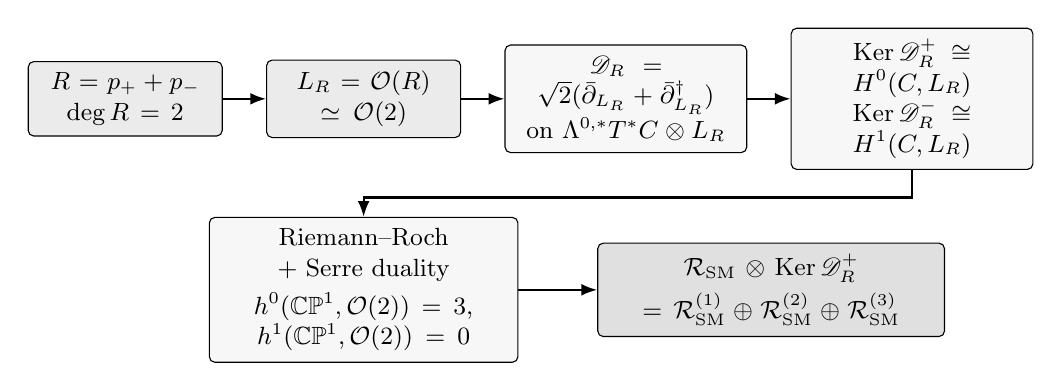
\begin{tikzpicture}[node distance=0.65cm and 0.55cm]
\node[psltinput, text width=0.18\linewidth] (div) {\(R=p_+ + p_-\)\\\(\deg R=2\)};
\node[psltinput, text width=0.18\linewidth, right=of div] (bundle) {\(L_R=\cO(R)\)\\\(\simeq\cO(2)\)};
\node[psltbox, text width=0.23\linewidth, right=of bundle] (dirac) {\(\scrD_R=\sqrt2(\bar\partial_{L_R}+\bar\partial_{L_R}^{\dagger})\)\\on \(\Lambda^{0,*}T^*C\otimes L_R\)};
\node[psltbox, text width=0.23\linewidth, right=of dirac] (hodge2) {\(\Ker\scrD_R^+\cong H^0(C,L_R)\)\\\(\Ker\scrD_R^-\cong H^1(C,L_R)\)};
\draw[psltarrow] (div) -- (bundle);
\draw[psltarrow] (bundle) -- (dirac);
\draw[psltarrow] (dirac) -- (hodge2);

\node[psltbox, text width=0.30\linewidth, below=1.0cm of bundle] (rr) {Riemann--Roch + Serre duality\\[1mm]\(h^0(\CP^1,\cO(2))=3\), \(\ h^1(\CP^1,\cO(2))=0\)};
\node[psltoutput, text width=0.34\linewidth, right=1.0cm of rr] (families) {\(\cR_{\rm SM}\otimes\Ker\scrD_R^+\)\\[1mm]\(=\cR_{\rm SM}^{(1)}\oplus\cR_{\rm SM}^{(2)}\oplus\cR_{\rm SM}^{(3)}\)};
\draw[psltarrow] (hodge2.south) -- ++(0,-0.35) -| (rr.north);
\draw[psltarrow] (rr) -- (families);
\end{tikzpicture}
}
\caption{Spin\(^c\) index-theoretic origin of the three protected families.
The two-center divisor fixes \(L_R=\cO(2)\).
The protected internal fermion operator is the Spin\(^c\) Dolbeault--Dirac operator, whose positive and negative kernels are identified by Hodge theory with \(H^0(C,L_R)\) and \(H^1(C,L_R)\).
For \(C=\CP^1\), Riemann--Roch and Serre duality give \(h^0=3\) and \(h^1=0\), so the positive internal zero-mode space produces three four-dimensional SM chiral family copies.}
\label{fig:index_chain}
\end{figure}

\begin{figure}[t]
\centering
\resizebox{\linewidth}{!}{%
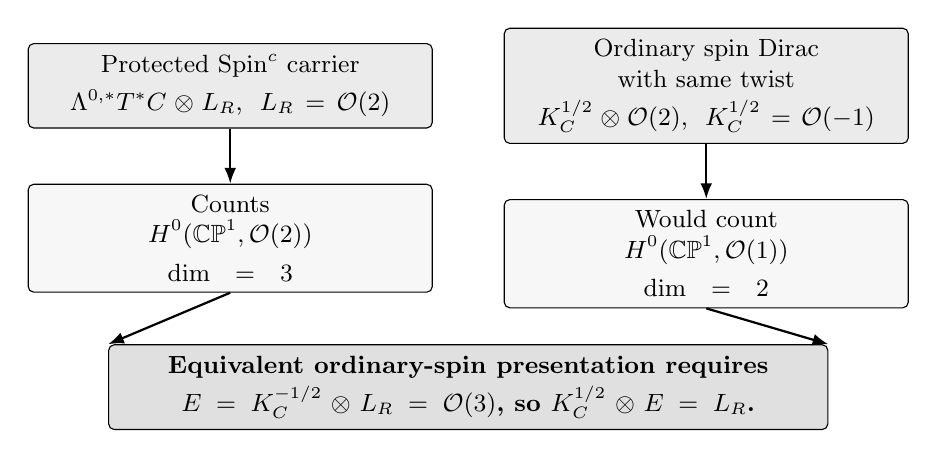
\begin{tikzpicture}[node distance=0.7cm and 0.9cm]
\node[psltinput, text width=0.40\linewidth] (spinc) {Protected Spin\(^c\) carrier\\[1mm]\(\Lambda^{0,*}T^*C\otimes L_R\), \(\ L_R=\cO(2)\)};
\node[psltinput, text width=0.40\linewidth, right=of spinc] (spin) {Ordinary spin Dirac with same twist\\[1mm]\(K_C^{1/2}\otimes\cO(2)\), \(\ K_C^{1/2}=\cO(-1)\)};

\node[psltbox, text width=0.40\linewidth, below=of spinc] (spinc_count) {Counts\\\(\displaystyle H^0(\CP^1,\cO(2))\)\\[1mm]\(\dim=3\)};
\node[psltbox, text width=0.40\linewidth, below=of spin] (spin_count) {Would count\\\(\displaystyle H^0(\CP^1,\cO(1))\)\\[1mm]\(\dim=2\)};
\draw[psltarrow] (spinc) -- (spinc_count);
\draw[psltarrow] (spin) -- (spin_count);

\node[psltoutput, text width=0.73\linewidth] (equiv) at ($(spinc_count.south)!0.5!(spin_count.south)+(0,-1.1cm)$) {Equivalent ordinary-spin presentation requires\\[1mm]\(E=K_C^{-1/2}\otimes L_R=\cO(3)\), so \(K_C^{1/2}\otimes E=L_R\).};
\draw[psltarrow] (spinc_count.south) -- (equiv.north west);
\draw[psltarrow] (spin_count.south) -- (equiv.north east);
\end{tikzpicture}
}
\caption{Why the Spin\(^c\) Dolbeault--Dirac representative is essential.
The protected sector used here is the canonical Spin\(^c\) bundle \(\Lambda^{0,*}T^*C\) twisted by \(L_R=\cO(2)\), and it counts \(H^0(\CP^1,\cO(2))\), giving three positive zero modes.
An ordinary spin Dirac operator on \(\CP^1\) includes \(K_C^{1/2}=\cO(-1)\); twisting it only by \(\cO(2)\) would count \(H^0(\CP^1,\cO(1))\), which is two-dimensional.
Thus the Spin\(^c\) carrier is part of the stated protected sector, not an interchangeable notation.}
\label{fig:spinc_vs_spin}
\end{figure}
\FloatBarrier

% ============================================================
\section{Three-Generation Theorem}
\label{sec:three_generation_theorem}

\begin{remark}[Assumption boundary]
The theorem below proves the multiplicity of unpaired SM-charged chiral zero modes inside the protected PSLT generation sector specified by \((C,R,L_R,\scrD_R)\).
It does not derive the two-center projection data or the protected carrier from a UV-complete compactification.
Those are model inputs; the statement proved here is the resulting Spin\(^c\) index theorem.
\end{remark}

\begin{theorem}[PSLT Spin\(^c\) three-generation theorem]
\label{thm:three_gen}
Let \(C=\CP^1\), \(R=p_+ + p_-\), and \(L_R=\cO(R)\simeq\cO(2)\).
Let the SM-charged generation carrier be
\[
\cR_{\rm SM}\otimes(\Lambda^{0,*}T^*C\otimes L_R),
\]
with internal operator \(\scrD_R\) as in Eq.~\eqref{eq:Dolbeault_Dirac}.
Assume the product Dirac action is Eq.~\eqref{eq:product_fermion_action}, the product chirality is Eq.~\eqref{eq:product_dirac}, every other SM-charged internal sector satisfies the full vectorlike gap condition of Eq.~\eqref{eq:vec_no_kernel} or Eq.~\eqref{eq:vectorlike_gap_condition}, and all remaining chiral sectors are SM-neutral.
Then the low-energy four-dimensional chiral SM spectrum contains exactly three unpaired SM-charged chiral generations:
\begin{equation}
N_{\rm gen}
=
\dim\Ker\scrD_R^+
-\dim\Ker\scrD_R^-
=3.
\label{eq:Ngen_index}
\end{equation}
Moreover, since \(\Ker\scrD_R^-=0\), the positive internal zero-mode space itself is three-dimensional.
\end{theorem}

\begin{proof}
Riemann--Roch for a line bundle \(L\) on a compact Riemann surface gives \cite{Hartshorne1977,GriffithsHarris1978,Forster1981}
\begin{equation}
h^0(C,L)-h^1(C,L)=\deg L+1-g(C).
\end{equation}
For \(C=\CP^1\), \(g(C)=0\).
Because \(R=p_+ + p_-\), \(\deg L_R=2\).
Therefore
\begin{equation}
h^0(C,L_R)-h^1(C,L_R)=3.
\label{eq:rr_index}
\end{equation}
Serre duality gives
\begin{equation}
h^1(C,L_R)
=
h^0(C,K_C\otimes L_R^{-1}).
\end{equation}
On \(\CP^1\),
\begin{equation}
K_C=\cO(-2),
\qquad
L_R^{-1}=\cO(-2),
\end{equation}
so
\begin{equation}
K_C\otimes L_R^{-1}=\cO(-4).
\end{equation}
A negative-degree line bundle on \(\CP^1\) has no nonzero holomorphic sections.
Thus
\begin{equation}
h^1(C,L_R)=0,
\qquad
h^0(C,L_R)=3.
\end{equation}
Using Eq.~\eqref{eq:hodge_kernel},
\begin{equation}
\dim\Ker\scrD_R^+=3,
\qquad
\dim\Ker\scrD_R^-=0.
\end{equation}
The product Dirac reduction in Eqs.~\eqref{eq:product_dirac}--\eqref{eq:internal_zero_mode_conditions} turns these internal zero modes into massless four-dimensional Weyl fermions.
The stated exclusivity assumption prevents additional nonzero-index SM-charged generation sectors, while the vectorlike gap condition removes unpaired massless SM-charged vectorlike exotics.
\end{proof}

In an affine coordinate \(\zeta\) on \(\CP^1\),
\begin{equation}
H^0(\CP^1,\cO(2))
=
\Span\{1,\zeta,\zeta^2\}.
\label{eq:holomorphic_basis}
\end{equation}
This span is only a vector space until a physical basis is chosen.
The family count is basis-independent; the labels \(N=1,2,3\) require a canonical Hermitian operator.

% ============================================================
\section{Canonical Generation Basis}
\label{sec:canonical_basis}

The two branch points alone determine the divisor and the family count, but a physical basis also needs the normalization of the affine coordinate on \(C\).
Placing \(p_+\) at \(0\) and \(p_-\) at \(\infty\) leaves the residual freedom \(\zeta_R\mapsto a\zeta_R\).
In PSLT this freedom is fixed by the two-center projection map from the spatial chart to the compact projection surface.

\subsection{Projection map and coordinate normalization}
\label{sec:projection_map}

Let \((\rho,z_{\rm ax},\varphi)\) be cylindrical coordinates on \(\mathbb R^3\), with the ordered centers
\begin{equation}
x_\pm:\quad \rho=0,\qquad z_{\rm ax}=\pm D/2.
\label{eq:spatial_centers}
\end{equation}
With regulator \(\varepsilon>0\), define
\begin{equation}
r_\pm
=
\sqrt{\rho^2+(z_{\rm ax}\mp D/2)^2+\varepsilon^2}.
\label{eq:rpm_projection}
\end{equation}
The physical affine coordinate is
\begin{equation}
\boxed{
\zeta_R(\rho,z_{\rm ax},\varphi;D,\varepsilon)
=
\left(\frac{r_+}{r_-}\right)^{1/2}\ee^{\ii\varphi}.
}
\label{eq:zeta_projection}
\end{equation}
Strictly, Eq.~\eqref{eq:zeta_projection} is a cylindrical-coordinate representative on
\(\mathbb R^3\setminus A_{\rm ax}\), where
\begin{equation}
A_{\rm ax}:=\{\rho=0\},
\end{equation}
because the angular coordinate \(\varphi\) is undefined on the axis.
The axial set has zero measure with respect to
\(\dd\mu_{\rm cyl}=\rho\,\dd\rho\,\dd z_{\rm ax}\,\dd\varphi\), so the pullback
construction used in the visibility integrals may be read in an \(L^2\)-almost-everywhere sense.
Equivalently, one may smooth the axial phase and take the regularized limit.
With this convention, we write the projection map as a map from the spatial chart:
\begin{equation}
\boxed{
\pi_D:\mathbb R^3\longrightarrow C\simeq\CP^1,
\qquad
\pi_D(\rho,z_{\rm ax},\varphi)
=
[1:\zeta_R(\rho,z_{\rm ax},\varphi;D,\varepsilon)].
}
\label{eq:piD_def}
\end{equation}
In the collapsed-core limit \(\varepsilon\to0\),
\begin{equation}
\pi_D(x_+)=p_+=[1:0],
\qquad
\pi_D(x_-)=p_-=[0:1].
\label{eq:piD_centers}
\end{equation}
For finite \(\varepsilon\), the source cores are mapped to regulated neighborhoods of the branch points.
The normalization is fixed by the midplane condition
\begin{equation}
z_{\rm ax}=0
\quad\Longrightarrow\quad
|\zeta_R|=1,
\label{eq:zeta_midplane}
\end{equation}
and the residual \(U(1)\) phase is fixed by the origin of the axial angle \(\varphi\).
Thus the earlier scale freedom \(\zeta_R\mapsto a\zeta_R\) is removed by the physical projection geometry rather than by an arbitrary Gram--Schmidt convention.

\subsection{Toeplitz basis}
\label{sec:toeplitz_basis}

Let \(P_R\) be the Bergman projector from \(L^2(C,L_R)\) onto \(H^0(C,L_R)\), using the Fubini--Study metric on \(C=\CP^1\) and the induced Hermitian metric on \(L_R\).
Using the coordinate \(\zeta_R\) fixed by Eq.~\eqref{eq:zeta_projection}, the associated axial moment-map function is
\begin{equation}
\mu_R(\zeta_R,\bar\zeta_R)
=
\frac{|\zeta_R|^2-1}{|\zeta_R|^2+1}.
\label{eq:moment_map}
\end{equation}
Let \(M_{\mu_R}\) denote multiplication by \(\mu_R\).
Define the finite-dimensional Toeplitz operator on \(H^0(C,L_R)\) by
\begin{equation}
\boxed{
\mathcal T_R=P_RM_{\mu_R}P_R
}
\label{eq:Toeplitz}
\end{equation}
This is a finite-dimensional Toeplitz quantization of the axial moment-map observable \cite{BordemannMeinrenkenSchlichenmaier1994}.
The generation basis is defined by
\begin{equation}
\mathcal T_Ru_N=\tau_Nu_N,
\qquad
u_N\in H^0(C,L_R),
\qquad
N=1,2,3.
\label{eq:uN_basis}
\end{equation}
For the symmetric two-center placement and the standard Fubini--Study/Bergman inner product, this basis is equivalent, up to normalization and ordering, to the spin-one monomial basis
\begin{equation}
1,\qquad \zeta,\qquad \zeta^2.
\end{equation}
In this symmetric realization \(\mathcal T_R\) is diagonal in the monomial basis and has three distinct axial weights; after the orientation of the ordered pair \((p_+,p_-)\) is fixed, it canonically orders the three one-dimensional eigenspaces.
The Toeplitz definition is the physical statement for labeling the already three-dimensional protected space; it is not a substitute for the Riemann--Roch and Serre-duality dimension argument.
The monomial basis is only a convenient coordinate representation.

\FloatBarrier
\begin{figure}[t]
\centering
\resizebox{\linewidth}{!}{%
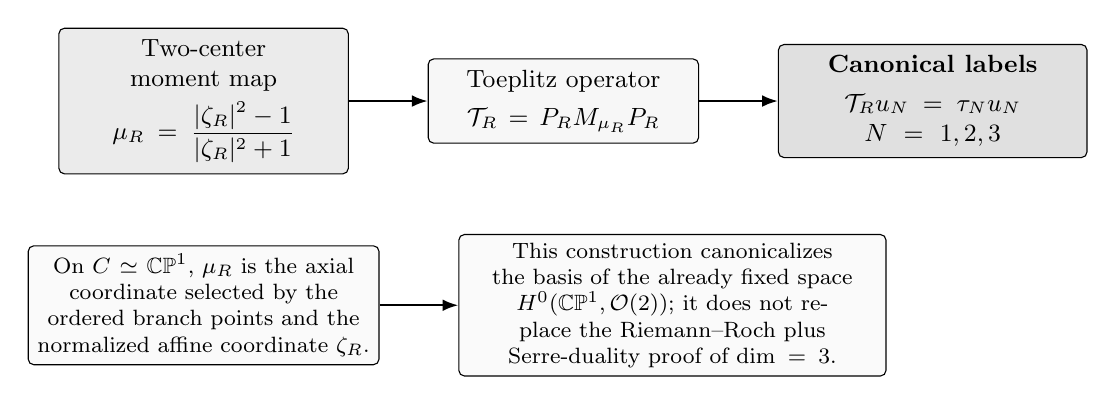
\begin{tikzpicture}[node distance=0.85cm and 1.0cm]
\node[psltinput, text width=0.28\linewidth] (moment) {Two-center moment map\\[1mm]\(\displaystyle \mu_R=\frac{|\zeta_R|^2-1}{|\zeta_R|^2+1}\)};
\node[psltbox, text width=0.26\linewidth, right=of moment] (toeplitz) {Toeplitz operator\\[1mm]\(\mathcal T_R=P_RM_{\mu_R}P_R\)};
\node[psltoutput, text width=0.30\linewidth, right=of toeplitz] (basis) {Canonical labels\\[1mm]\(\mathcal T_Ru_N=\tau_Nu_N\)\\\(N=1,2,3\)};
\draw[psltarrow] (moment) -- (toeplitz);
\draw[psltarrow] (toeplitz) -- (basis);

\node[psltthin, text width=0.35\linewidth, below=0.9cm of moment] (sphere) {On \(C\simeq\CP^1\), \(\mu_R\) is the axial coordinate selected by the ordered branch points and the normalized affine coordinate \(\zeta_R\).};
\node[psltthin, text width=0.43\linewidth, right=of sphere] (countnote) {This construction canonicalizes the basis of the already fixed space \(H^0(\CP^1,\cO(2))\); it does not replace the Riemann--Roch plus Serre-duality proof of \(\dim=3\).};
\draw[psltarrow] (sphere) -- (countnote);
\end{tikzpicture}
}
\caption{Canonical family labels from the two-center Toeplitz operator.
The family count \(\dim H^0(\CP^1,\cO(2))=3\) is basis-independent, but physical labels require a canonical Hermitian operator.
The two-center projection fixes the affine coordinate \(\zeta_R\), hence the axial moment-map function \(\mu_R\).
Projecting multiplication by \(\mu_R\) onto the protected holomorphic section space gives the Toeplitz operator \(\mathcal T_R=P_RM_{\mu_R}P_R\).
Its eigenvectors define the canonical generation basis, equivalent for the symmetric two-center placement to the spin-one monomial basis \(1,\zeta,\zeta^2\) up to normalization and ordering.}
\label{fig:toeplitz_basis}
\end{figure}
\FloatBarrier

% ============================================================
\section{Two-Center Conformal Geometry}
\label{sec:two_center_geometry}

The two-center conformal factor is obtained in the static sector.
The covariant effective term \(S_\Omega^{\rm cov}\) in Eq.~\eqref{eq:parent_action} is not specified by the spatial expression below; rather, under the static two-center ansatz it reduces to the three-dimensional variational energy functional
\begin{equation}
E_\Omega
=
\frac{\kappa}{2}
\int_{\mathbb R^3}\dd^3x\,|\nabla\Omega|^2
-4\pi\kappa
\int_{\mathbb R^3}\dd^3x\,\sigma(x)(\Omega-1),
\label{eq:E_Omega}
\end{equation}
with
\begin{equation}
\sigma(x)
=
a\left[\rho_\varepsilon(x-x_+)+\rho_\varepsilon(x-x_-)\right].
\label{eq:sigma}
\end{equation}
Variation gives
\begin{equation}
\delta E_\Omega
=
-\kappa
\int_{\mathbb R^3}\dd^3x\,
\left(\nabla^2\Omega+4\pi\sigma\right)\delta\Omega,
\end{equation}
hence
\begin{equation}
\boxed{
\nabla^2\Omega=-4\pi\sigma.
}
\label{eq:Poisson}
\end{equation}
Let \((\rho,z_{\rm ax},\varphi)\) be cylindrical coordinates on \(\mathbb R^3\), with centers at
\begin{equation}
x_\pm:\quad \rho=0,\qquad z_{\rm ax}=\pm D/2.
\end{equation}
For
\begin{equation}
\rho_\varepsilon(r)
=
\frac{3\varepsilon^2}{4\pi(r^2+\varepsilon^2)^{5/2}},
\qquad
\int_{\mathbb R^3}\dd^3x\,\rho_\varepsilon=1,
\end{equation}
the asymptotically flat solution is
\begin{equation}
\boxed{
\Omega(\rho,z_{\rm ax};D)
=
1+a\left(\frac1{r_+}+\frac1{r_-}\right),
\qquad
r_\pm
=
\sqrt{\rho^2+(z_{\rm ax}\mp D/2)^2+\varepsilon^2}.
}
\label{eq:Omega_solution}
\end{equation}

% ============================================================
\section{Geometry-to-Spectrum Map}
\label{sec:geometry_spectrum}

We use the mostly-plus convention \cite{Nakahara2003,BirrellDavies1982}
\begin{equation}
\eta_{\mu\nu}=\diag(-,+,+,+),
\qquad
\Box_\eta=-\partial_t^2+\nabla^2,
\label{eq:signature}
\end{equation}
and the curvature convention
\begin{equation}
R^\rho{}_{\sigma\mu\nu}
=
\partial_\mu\Gamma^\rho_{\nu\sigma}
-\partial_\nu\Gamma^\rho_{\mu\sigma}
+\Gamma^\rho_{\mu\lambda}\Gamma^\lambda_{\nu\sigma}
-\Gamma^\rho_{\nu\lambda}\Gamma^\lambda_{\mu\sigma}.
\label{eq:curvature_convention}
\end{equation}
For the static conformally flat metric
\begin{equation}
g_{\mu\nu}=\Omega^2(x)\eta_{\mu\nu},
\end{equation}
this gives
\begin{equation}
R=-6\Omega^{-3}\nabla^2\Omega.
\label{eq:Ricci_scalar}
\end{equation}
Consider
\begin{equation}
(\Box_g-m_0^2-\xi R)\Phi=0,
\qquad
\Phi(t,x)=\ee^{-\ii\omega t}\Omega^{-1}(x)\psi(x).
\end{equation}
Using
\begin{equation}
\left(\Box_g-\frac16R\right)(\Omega^{-1}\psi)
=
\Omega^{-3}\Box_\eta\psi,
\end{equation}
one obtains
\begin{equation}
\left[
-\nabla^2
+m_0^2\Omega^2
+(1-6\xi)\Omega^{-1}\nabla^2\Omega
\right]\psi
=
\omega^2\psi.
\label{eq:scalar_operator_derived}
\end{equation}
Define
\begin{equation}
V_{\rm eff}
=
m_0^2\Omega^2
+(1-6\xi)\Omega^{-1}\nabla^2\Omega.
\label{eq:Veff}
\end{equation}
Then
\begin{equation}
\boxed{
[-\nabla^2+V_{\rm eff}]\psi_n=\omega_n^2\psi_n.
}
\label{eq:schrodinger}
\end{equation}
This scalar spectral problem governs formation barriers and visible overlap profiles.
It does not determine the number of chiral SM generations; that number is fixed by \(\scrD_R\).

% ============================================================
\section{Degeneracy, Kinetics, Visibility, and Formation}
\label{sec:probability_modules}

\begin{figure}[t]
\centering
\resizebox{\linewidth}{!}{%
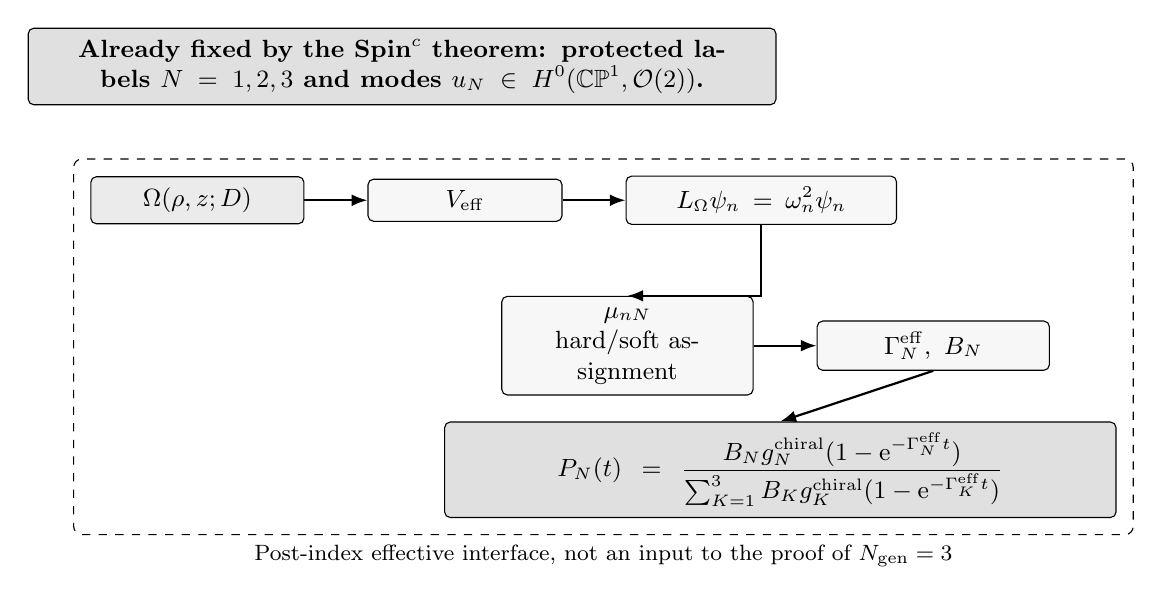
\begin{tikzpicture}[node distance=0.75cm and 0.8cm]
\node[psltoutput, text width=0.76\linewidth] (fixed) {Already fixed by the Spin\(^c\) theorem: protected labels \(N=1,2,3\) and modes \(u_N\in H^0(\CP^1,\cO(2))\).};

\node[psltinput, text width=0.20\linewidth, below=0.9cm of fixed, xshift=-2.6cm] (omega) {\(\Omega(\rho,z;D)\)};
\node[psltbox, text width=0.18\linewidth, right=of omega] (veff) {\(V_{\rm eff}\)};
\node[psltbox, text width=0.26\linewidth, right=of veff] (scalar_modes) {\(L_\Omega\psi_n=\omega_n^2\psi_n\)};
\draw[psltarrow] (omega) -- (veff);
\draw[psltarrow] (veff) -- (scalar_modes);

\node[psltbox, text width=0.24\linewidth, below=0.9cm of scalar_modes, xshift=-1.7cm] (locking) {\(\mu_{nN}\)\\hard/soft assignment};
\node[psltbox, text width=0.22\linewidth, right=of locking] (rates2) {\(\Gamma_N^{\rm eff},\ B_N\)};
\draw[psltarrow] (scalar_modes.south) |- (locking.north);
\draw[psltarrow] (locking) -- (rates2);

\node[psltoutput, text width=0.68\linewidth] (prob) at ($(locking.south)!0.5!(rates2.south)+(0,-1.1cm)$) {\(\displaystyle
P_N(t)=
\frac{B_Ng_N^{\rm chiral}(1-\ee^{-\Gamma_N^{\rm eff}t})}
{\sum_{K=1}^3B_Kg_K^{\rm chiral}(1-\ee^{-\Gamma_K^{\rm eff}t})}\)};
\draw[psltarrow] (rates2.south) -- (prob.north);
\node[psltdash, fit=(omega)(veff)(scalar_modes)(locking)(rates2)(prob), label={[font=\footnotesize]below:Post-index effective interface, not an input to the proof of \(N_{\rm gen}=3\)}] {};
\end{tikzpicture}
}
\caption{Post-index scalar spectral interface for formation and visibility.
After the Spin\(^c\) index theorem has fixed the protected generation space to three modes, the two-center scalar geometry supplies an effective interface for profiles, rates, and visible overlaps.
The conformal factor \(\Omega\) determines \(V_{\rm eff}\), whose scalar eigenmodes \(\psi_n\) are connected to the protected labels only through scalarization weights and hard/soft assignment.
The probability law \(P_N(t)\) describes post-index formation and visibility of \(N=1,2,3\); it is not an additional input to the proof of the family multiplicity.}
\label{fig:post_index_interface}
\end{figure}
\FloatBarrier

The structures in this section are an effective formation/visibility model built on the Spin\(^c\) generation theorem.
They use scalar spectral data and two-center collective coordinates to parametrize rates and overlaps; they do not supply an independent proof of the number of chiral SM generations.
The interface data used below are precisely \(\mathfrak D_{\rm int}(D)\) from Eq.~\eqref{eq:interface_data}; changing them changes the effective formation/visibility model, not the Spin\(^c\) multiplicity result.

For the protected chiral sector, let \(\Pi_N=|u_N\rangle\langle u_N|\) be the projector onto the Toeplitz eigenmode \(u_N\).
The chiral degeneracy is
\begin{equation}
g_N^{\rm chiral}
=
\Tr_{\cH_{\rm gen}}\Pi_N,
\qquad
\cH_{\rm gen}=H^0(\CP^1,\cO(2)).
\end{equation}
Thus
\begin{equation}
\boxed{
g_1^{\rm chiral}=g_2^{\rm chiral}=g_3^{\rm chiral}=1,
\qquad
g_{N\ge4}^{\rm chiral}=0.
}
\label{eq:gN}
\end{equation}

\subsection{Generation-to-spatial mode assignment}
\label{sec:mode_locking}

The protected generation basis \(u_N\in H^0(C,L_R)\) and the scalar spatial eigenmodes \(\psi_n\) of Eq.~\eqref{eq:schrodinger} are not the same objects.
The former are Spin\(^c\) zero modes on \(C\); the latter are eigenfunctions of a Schr\"odinger operator on the spatial two-center chart.
We reserve \(N=1,2,3\) for protected generation labels and \(n\) for scalar spectral labels.
Define
\begin{equation}
\cH_{\rm gen}
=
H^0(C,L_R),
\qquad
\cH_\Omega(D)
=
L^2(\mathbb R^3,\dd\mu_{\rm cyl}),
\qquad
\dd\mu_{\rm cyl}
=
\rho\,\dd\rho\,\dd z_{\rm ax}\,\dd\varphi,
\label{eq:gen_scalar_spaces}
\end{equation}
and
\begin{equation}
L_\Omega(D):=-\nabla^2+V_{\rm eff}(\cdot;D),
\qquad
L_\Omega(D)\psi_n(\cdot;D)
=
\omega_n^2(D)\psi_n(\cdot;D).
\label{eq:LOmega_modes}
\end{equation}
We use the Friedrichs self-adjoint realization of \(L_\Omega(D)\) associated
with the semibounded quadratic form of Eq.~\eqref{eq:LOmega_modes} on
\(\cH_\Omega(D)\), after the regulated two-center potential
\(V_{\rm eff}(\cdot;D)\) has been fixed.
In finite-volume numerical applications, \(L_\Omega(D)\) denotes the
corresponding self-adjoint realization with the stated boundary conditions.
The notation \(\dd E_\lambda(D)\) below is the projection-valued spectral
measure of this self-adjoint operator \cite{ReedSimon4}.
The projection map \(\pi_D\) pulls the generation bundle to the spatial chart:
\begin{equation}
\widehat L_R:=\pi_D^*L_R,
\qquad
\widehat h_R:=\pi_D^*h_R,
\qquad
\widehat u:=\pi_D^*u
\in
\Gamma(\mathbb R^3,\widehat L_R).
\label{eq:pullback_generation_bundle}
\end{equation}
To attach scalar barrier data to a protected generation, introduce the linear raw scalarization operator
\begin{equation}
\boxed{
\widetilde{\mathcal C}_D:\cH_{\rm gen}\longrightarrow \cH_\Omega(D),
\qquad
\widetilde{\mathcal C}_Du
=
w_D^{1/2}\,
\left\langle
\mathfrak j_D,
\pi_D^*u
\right\rangle_{\widehat h_R}.
}
\label{eq:scalarization_operator}
\end{equation}
Here \(\mathfrak j_D\in\Gamma(\mathbb R^3,\widehat L_R)\) is the locking/probe section supplied by the two-center projection data, and \(w_D\ge0\) is a scalar density weight.
With our convention that the Hermitian pairing is antilinear in the first entry and linear in the second, \(\widetilde{\mathcal C}_D\) is linear in \(u\).
The raw scalar profile is assumed nonzero on the protected modes \(u_N\).
The normalized profile map is the generally nonlinear map
\begin{equation}
\boxed{
c_D(u)
=
\frac{\widetilde{\mathcal C}_Du}
{\|\widetilde{\mathcal C}_Du\|_{\cH_\Omega(D)}}.
}
\label{eq:normalized_scalar_profile}
\end{equation}
The spectral weights of a generation mode against scalar eigenmodes are
\begin{equation}
\boxed{
\mu_{nN}(D)
=
\left|
\left\langle
\psi_n(\cdot;D),
c_D(u_N)
\right\rangle_{\cH_\Omega(D)}
\right|^2.
}
\label{eq:spectral_weights}
\end{equation}
For a normalized discrete scalar spectral resolution, \(\sum_n\mu_{nN}=1\).
If the scalar operator has a continuous component, Eq.~\eqref{eq:spectral_weights} is replaced by the projection-valued spectral measure
\begin{equation}
\dd\mu_N^D(\lambda)
=
\left\|
\dd E_\lambda(D)\,c_D(u_N)
\right\|_{\cH_\Omega(D)}^2.
\label{eq:spectral_measure}
\end{equation}
Only when a unique scalar mode dominates do we define a hard mode-locking map.
The condition is
\begin{equation}
n(N;D)
=
\operatorname*{arg\,max}_{n}\mu_{nN}(D),
\qquad
\mu_{n(N;D),N}(D)
-
\sup_{m\ne n(N;D)}\mu_{mN}(D)
\ge
\Delta_{\rm lock}>0.
\label{eq:locking_gap}
\end{equation}
In that regime,
\begin{equation}
\mathcal I_D(u_N):=\psi_{n(N;D)}(\cdot;D),
\qquad
\psi_N^{\rm lock}:=\psi_{n(N;D)},
\qquad
\omega_N(D):=\omega_{n(N;D)}(D).
\label{eq:hard_locking_map}
\end{equation}
If Eq.~\eqref{eq:locking_gap} fails, the generation must be assigned scalar data softly:
\begin{equation}
\Gamma_N^{\rm soft}(D,\eta)
=
\sum_n\mu_{nN}(D)\,\Gamma_n(D,\eta),
\label{eq:soft_rate_discrete}
\end{equation}
or, for a continuous spectral component,
\begin{equation}
\Gamma_N^{\rm soft}(D,\eta)
=
\int \Gamma(\lambda;D,\eta)\,\dd\mu_N^D(\lambda).
\label{eq:soft_rate_continuous}
\end{equation}
Here \(\Gamma_n\) is the scalar-mode formation rate for the \(n\)th eigenmode, computed by the same two-center Schur/WKB construction.
Thus the Spin\(^c\) theorem fixes \(u_N\), while \(\widetilde{\mathcal C}_D\), \(c_D\), \(\mu_{nN}\), and, only under Eq.~\eqref{eq:locking_gap}, \(\mathcal I_D\), supply the scalar formation interface.
All hard-locking quantities \(\omega_N\), \(\Gamma_N\), and \(|N,\pm\rangle\) below are understood only after Eq.~\eqref{eq:locking_gap}; the final probability law is written with \(\Gamma_N^{\rm eff}\) to cover both the hard-locking and soft-assignment regimes.

For kinetics in the hard-locking regime, the locked scalar mode \(\psi_N^{\rm lock}\) and the two centers define a collective-coordinate subspace
\begin{equation}
\cC_N=\Span\{|N,+\rangle,\ |N,-\rangle\}.
\end{equation}
Let \(P_N^{\rm cc}\) project onto \(\cC_N\), \(Q_N^{\rm cc}=1-P_N^{\rm cc}\), and let \(\cK_N(D,\eta)\) be the Euclidean fluctuation operator in this sector.
The dimensionless parameter \(\eta\) denotes the two-center overlap controlling kinetic mixing.
For the regulated source model, we take
\begin{equation}
\boxed{
\eta(D,\varepsilon)
=
\int_{\mathbb R^3}\dd^3x\,
\sqrt{
\rho_\varepsilon(x-x_+)\rho_\varepsilon(x-x_-)
},
\qquad
0\le \eta\le1.
}
\label{eq:eta_def}
\end{equation}
Since \(\rho_\varepsilon\) is normalized, Eq.~\eqref{eq:eta_def} is the Hellinger affinity of the two regulated source densities.
The bound \(0\le\eta\le1\) follows from Cauchy--Schwarz, with \(\eta=1\) only for coincident identical profiles.
It enters the fluctuation operator, WKB prefactors, and center mixing coefficient:
\begin{equation}
\cK_N=\cK_N(D,\eta),
\qquad
A_{N,\pm}=A_{N,\pm}(D,\eta),
\qquad
\chi_N=\chi_N(D,\eta).
\label{eq:eta_dependencies}
\end{equation}
The Feshbach--Schur step assumes a gap on the eliminated complement:
\begin{equation}
0\notin
\operatorname{Spec}
\left(
Q_N^{\rm cc}\cK_N(D,\eta)Q_N^{\rm cc}
\right).
\label{eq:schur_gap_assumption}
\end{equation}
If this gap closes, the inverse below must be replaced by the corresponding reduced resolvent or pseudoinverse.
Under Eq.~\eqref{eq:schur_gap_assumption}, the Feshbach--Schur effective matrix is \cite{Feshbach1958}
\begin{equation}
\cM_N
=
P_N^{\rm cc}\cK_NP_N^{\rm cc}
-P_N^{\rm cc}\cK_NQ_N^{\rm cc}
(Q_N^{\rm cc}\cK_NQ_N^{\rm cc})^{-1}
Q_N^{\rm cc}\cK_NP_N^{\rm cc}.
\label{eq:Schur_matrix}
\end{equation}
In the two-center basis,
\begin{equation}
\cM_N
=
\begin{pmatrix}
\gamma_{N,+} &
\chi_N\sqrt{\gamma_{N,+}\gamma_{N,-}}\\
\chi_N\sqrt{\gamma_{N,+}\gamma_{N,-}}&
\gamma_{N,-}
\end{pmatrix},
\end{equation}
with WKB channel factors
\begin{equation}
\gamma_{N,\pm}
=
A_{N,\pm}\exp[-2S_{N,\pm}^{\rm WKB}],
\qquad
S_{N,\pm}^{\rm WKB}
=
\int_{\cB_{N,\pm}}\dd s\,
\sqrt{\left(V_{\rm eff}(s)-\omega_N^2\right)_+}.
\label{eq:WKB}
\end{equation}
Here
\begin{equation}
\cB_{N,\pm}
=
\{s\text{ on the } \pm\text{ channel}:\ V_{\rm eff}(s)>\omega_N^2\},
\label{eq:wkb_barrier_region}
\end{equation}
and \((x)_+=\max\{x,0\}\).
The formation rate is
\begin{equation}
\boxed{
\Gamma_N(D,\eta)
=
\max\{0,\lambda_+(\cM_N(D,\eta))\},
}
\label{eq:Gamma}
\end{equation}
where
\begin{equation}
\lambda_+(\cM_N)
=
\frac{\gamma_{N,+}+\gamma_{N,-}}{2}
+\frac12
\sqrt{
(\gamma_{N,+}-\gamma_{N,-})^2
+4\chi_N^2\gamma_{N,+}\gamma_{N,-}
}.
\end{equation}

For visibility, use the same pullback bundle from Eq.~\eqref{eq:pullback_generation_bundle}.
For the \(N\)th generation, the spatial representative is the section
\begin{equation}
\widehat u_N:=\pi_D^*u_N
\in
\Gamma(\mathbb R^3,\widehat L_R),
\label{eq:uN_pullback}
\end{equation}
not a scalar function.
The visible kernel is correspondingly a bundle-valued source
\begin{equation}
\mathcal J_{\rm vis}(D,\varepsilon)
\in
\Gamma(\mathbb R^3,\widehat L_R).
\label{eq:Jvis_bundle}
\end{equation}
The \(\varphi\)-dependence is therefore not discarded; in axially reduced formulas it has already been projected into the selected angular channel and absorbed into the chosen representative of \(\mathcal J_{\rm vis}\) and the measure factor.
The conformal Dirac and Higgs fields scale as
\begin{equation}
\Psi=\Omega^{-3/2}\psi,
\qquad
H=\Omega^{-1}\phi.
\end{equation}
Hence
\begin{equation}
\sqrt{-g}\,\bar\Psi H\Psi
\propto
\Omega^4\cdot\Omega^{-3/2}\cdot\Omega^{-1}\cdot\Omega^{-3/2}
=
\Omega^0.
\label{eq:weyl_yukawa}
\end{equation}
A mode-resolved Yukawa overlap is the Hermitian pairing on the pullback bundle:
\begin{equation}
\boxed{
y_N^{\rm eff}(D,\varepsilon)
=
y_0
\int_{\mathbb R^3}
\left\langle
\widehat u_N(x;D,\varepsilon),
\mathcal J_{\rm vis}(x;D,\varepsilon)
\right\rangle_{\widehat h_R}
\dd\mu_{\rm cyl}(x),
}
\label{eq:y_eff}
\end{equation}
We use the convention that the Hermitian pairing is antilinear in the first entry.
With this mathematical convention, \(y_N^{\rm eff}\) is an antilinear amplitude in the generation vector \(u_N\).
This does not affect \(B_N\), which depends only on \(|y_N^{\rm eff}|^2\).
If \(y_N^{\rm eff}\) is later used as a phase-sensitive Yukawa or Wilson coefficient and one wants a convention linear in \(u_N\), one may equivalently use the opposite pairing order,
\(\int\langle\mathcal J_{\rm vis},\widehat u_N\rangle_{\widehat h_R}\,\dd\mu_{\rm cyl}\);
the normalized visibility \(B_N\) is unchanged.
In a local frame \(\widehat e_R=\pi_D^*e_R\), write
\begin{equation}
\widehat u_N=U_N\widehat e_R,
\qquad
\mathcal J_{\rm vis}=J_{\rm vis}\widehat e_R,
\qquad
\widehat h_R(\widehat e_R,\widehat e_R)=H_R.
\label{eq:local_visibility_frame}
\end{equation}
Then
\begin{equation}
\left\langle
\widehat u_N,
\mathcal J_{\rm vis}
\right\rangle_{\widehat h_R}
=
H_R\,\overline{U_N}\,J_{\rm vis}.
\label{eq:local_visibility_pairing}
\end{equation}
This is independent of the frame.
Indeed, under \(\widehat e_R'=g\,\widehat e_R\), with \(g:\mathbb R^3\to\mathbb C^*\),
\begin{equation}
U_N'=g^{-1}U_N,
\qquad
J_{\rm vis}'=g^{-1}J_{\rm vis},
\qquad
H_R'=|g|^2H_R,
\end{equation}
and hence
\begin{equation}
H_R'\,\overline{U_N'}\,J_{\rm vis}'
=
H_R\,\overline{U_N}\,J_{\rm vis}.
\label{eq:frame_invariance}
\end{equation}
The earlier scalar-looking formula is only this local trivialized representative:
\begin{equation}
\begin{aligned}
y_N^{\rm eff}(D,\varepsilon)
=\;&
y_0
\int_0^\infty \rho\,\dd\rho
\int_{-\infty}^{\infty}\dd z_{\rm ax}
\int_0^{2\pi}\dd\varphi\,
\overline{U_N(\rho,z_{\rm ax},\varphi;D,\varepsilon)}
\\
&\times
f_L(\rho,z_{\rm ax})
f_R(\rho,z_{\rm ax})
W_{\rm frame}(\rho,z_{\rm ax},\varphi;D,\varepsilon).
\end{aligned}
\label{eq:y_eff_local}
\end{equation}
Here \(W_{\rm frame}\) is not an additional invariant object; it denotes the local representative of the bundle frame, Hermitian metric \(H_R\), visible source \(J_{\rm vis}\), angular-channel projection, Jacobian convention, and any remaining complex-conjugation convention.
When the visible kernel has already been reduced to an \(m=0\) axial channel, Eq.~\eqref{eq:y_eff_local} reduces to the earlier \(2\pi\rho\,\dd\rho\,\dd z_{\rm ax}\) form with the angular integral included in \(W_{\rm frame}\).
The normalized visible weight is
\begin{equation}
\boxed{
B_N
=
\frac{|y_N^{\rm eff}|^2}
{\sum_{I=1}^{3}|y_I^{\rm eff}|^2}.
}
\label{eq:BN}
\end{equation}
We assume the visible kernel is not orthogonal to the entire protected generation space, so that
\begin{equation}
\sum_{I=1}^{3}|y_I^{\rm eff}|^2>0.
\label{eq:BN_denominator_nonzero}
\end{equation}
Under this nonzero-overlap condition the normalized weights \(B_N\) are well defined.
For the operator notation in the equivalent form, define the linear visible-overlap functional
\begin{equation}
\mathcal O_{\rm vis}:\cH_{\rm gen}\longrightarrow\mathbb C,
\qquad
(\mathcal O_{\rm vis}u)
=
y_0
\int_{\mathbb R^3}
\left\langle
\mathcal J_{\rm vis}(x;D,\varepsilon),
\pi_D^*u(x)
\right\rangle_{\widehat h_R}
\dd\mu_{\rm cyl}(x).
\label{eq:Ovis_def}
\end{equation}
This uses the opposite pairing order from Eq.~\eqref{eq:y_eff}, so it is linear in \(u\) under the stated Hermitian convention.
The two overlap conventions differ only by pairing order and conjugation convention and give
\begin{equation}
|\mathcal O_{\rm vis}u_N|^2=|y_N^{\rm eff}|^2.
\end{equation}
Thus \(\mathcal O_{\rm vis}^\dagger\mathcal O_{\rm vis}\) is the induced rank-one positive operator on \(\cH_{\rm gen}\), and equivalently
\begin{equation}
B_N
=
\frac{\langle u_N|\mathcal O_{\rm vis}^\dagger\mathcal O_{\rm vis}|u_N\rangle}
{\sum_{I=1}^{3}
\langle u_I|\mathcal O_{\rm vis}^\dagger\mathcal O_{\rm vis}|u_I\rangle}.
\end{equation}

Finally, at the coarse-grained effective level, define the rate used by the conditional probability law as
\begin{equation}
\Gamma_N^{\rm eff}(D,\eta)
=
\begin{cases}
\Gamma_N(D,\eta), & \text{in the hard-locking regime of Eq.~\eqref{eq:locking_gap}},\\
\Gamma_N^{\rm soft}(D,\eta), & \text{otherwise}.
\end{cases}
\label{eq:Gamma_eff}
\end{equation}
Assume the corresponding single-rate Markovian formation law
\begin{equation}
\frac{\dd p_N}{\dd t}=\Gamma_N^{\rm eff}(1-p_N),
\qquad
p_N(0)=0
\end{equation}
has solution
\begin{equation}
p_N(t)=1-\ee^{-\Gamma_N^{\rm eff}t}.
\end{equation}
Conditioning on the observation of one of the protected chiral layers gives
\begin{equation}
\boxed{
P_N(t;D,\eta)
=
\frac{
B_Ng_N^{\rm chiral}\left(1-\ee^{-\Gamma_N^{\rm eff}(D,\eta)t}\right)
}{
\sum_{K=1}^{3}
B_Kg_K^{\rm chiral}\left(1-\ee^{-\Gamma_K^{\rm eff}(D,\eta)t}\right)
}.
}
\label{eq:PN}
\end{equation}
Equation~\eqref{eq:PN} is understood for \(t>0\) and for parameter values for which the denominator is nonzero.
At \(t=0\), or if all effective formation rates vanish, the conditional observation probability is not defined.
When the rate-weighted denominator is nonzero, the right limit is
\begin{equation}
P_N(0^+;D,\eta)
=
\frac{
B_Ng_N^{\rm chiral}\Gamma_N^{\rm eff}(D,\eta)
}{
\sum_{K=1}^{3}
B_Kg_K^{\rm chiral}\Gamma_K^{\rm eff}(D,\eta)
}.
\label{eq:PN_zero_plus}
\end{equation}

% ============================================================
\section{Limitations and Outlook}
\label{sec:limitations_outlook}

The result should be read as a conditional field-theoretic and index-theoretic model, not as a complete theory of flavor.
Several inputs remain outside the theorem.
First, the paper assumes the PSLT two-center projection data \((C,R)\) rather than deriving \(C=\CP^1\) and \(R=p_+ + p_-\) from a UV-complete quantum-gravity vacuum.
Second, the protected SM-charged carrier \(\cR_{\rm SM}\otimes(\Lambda^{0,*}T^*C\otimes L_R)\) and the Spin\(^c\) Dolbeault representative are taken as the protected generation sector; the BPS remark provides a compatible motivation, not a universal vacuum-selection theorem.
Third, the exact three-family conclusion requires the stated exclusivity and gap assumptions for all additional SM-charged internal sectors.
Fourth, the theorem fixes the multiplicity of protected family copies but does not determine Yukawa hierarchies, CKM or PMNS mixing, neutrino masses, or the detailed spectrum of massive vectorlike states.

The scalar two-center spectral operator and the effective quantities \((g_N^{\rm chiral},\Gamma_N^{\rm eff},B_N,P_N)\) should therefore be viewed as a post-index phenomenological interface.
They can be used to assign formation rates and visible-sector overlaps to the three protected modes, but they are not inputs to the Spin\(^c\) proof of \(N_{\rm gen}=3\).
Future work would need to derive the projection data and protected carrier from a more microscopic PSLT or compactification construction, and then connect the overlap functional to realistic flavor textures.

% ============================================================
\section{Conclusion}
\label{sec:conclusion}

The two-center PSLT projection data determine the divisor \(R=p_+ + p_-\) and the line bundle \(L_R=\cO(R)\simeq\cO(2)\) on \(C=\CP^1\).
The SM-charged internal fermions are governed by the product Dirac action on \(M_4\times C\), with the internal Spin\(^c\) Dolbeault--Dirac operator acting on \(\Lambda^{0,*}T^*C\otimes L_R\).
The bundle \(L_R\) is the auxiliary Dolbeault twist, and the positive and negative internal zero modes are \(H^0(C,L_R)\) and \(H^1(C,L_R)\).
Riemann--Roch gives index three, and Serre duality gives \(H^1(C,L_R)=0\).
Thus, conditional on the PSLT two-center projection data and the stated gap/exclusivity assumptions, the protected SM-charged generation sector contributes exactly three low-energy chiral SM family copies, with no additional unpaired light SM-charged exotics arising from the allowed extra sectors.

After the raw scalarization operator \(\widetilde{\mathcal C}_D\), the normalized profile map \(c_D\), the spectral weights \(\mu_{nN}\), and, when the locking gap exists, the hard map \(\mathcal I_D:u_N\mapsto\psi_N^{\rm lock}\), the scalar two-center spectral operator and the quantities \((g_N^{\rm chiral},\Gamma_N^{\rm eff},B_N,P_N)\) define an effective model for how these three protected modes form and couple to the visible sector.
They are coarse-grained phenomenological structures on top of the Spin\(^c\) generation theorem, not substitutes for it.

\begin{acknowledgments}
The author reports no external funding for this work.
\end{acknowledgments}

\begin{thebibliography}{99}

\bibitem{AtiyahSinger1968}
M.~F.~Atiyah and I.~M.~Singer,
``The index of elliptic operators: I,''
Annals Math. \textbf{87}, 484 (1968).

\bibitem{Hartshorne1977}
R.~Hartshorne,
\textit{Algebraic Geometry},
Graduate Texts in Mathematics Vol.~52,
Springer (1977).

\bibitem{GriffithsHarris1978}
P.~Griffiths and J.~Harris,
\textit{Principles of Algebraic Geometry},
Wiley (1978).

\bibitem{Forster1981}
O.~Forster,
\textit{Lectures on Riemann Surfaces},
Graduate Texts in Mathematics Vol.~81,
Springer (1981).

\bibitem{LawsonMichelsohn1989}
H.~B.~Lawson and M.-L.~Michelsohn,
\textit{Spin Geometry},
Princeton University Press (1989).

\bibitem{Nakahara2003}
M.~Nakahara,
\textit{Geometry, Topology and Physics},
2nd ed.,
Institute of Physics Publishing (2003).

\bibitem{Bertlmann1996}
R.~A.~Bertlmann,
\textit{Anomalies in Quantum Field Theory},
Oxford University Press (1996).

\bibitem{Bilal2008}
A.~Bilal,
``Lectures on Anomalies,''
arXiv:0802.0634.

\bibitem{Witten1982SU2}
E.~Witten,
``An \(SU(2)\) anomaly,''
Phys. Lett. B \textbf{117}, 324 (1982).

\bibitem{Candelas1985}
P.~Candelas, G.~T.~Horowitz, A.~Strominger, and E.~Witten,
``Vacuum configurations for superstrings,''
Nucl. Phys. B \textbf{258}, 46 (1985).

\bibitem{Witten1986}
E.~Witten,
``New issues in manifolds of \(SU(3)\) holonomy,''
Nucl. Phys. B \textbf{268}, 79 (1986).

\bibitem{BraunHeOvrutPantev2005}
V.~Braun, Y.-H.~He, B.~A.~Ovrut, and T.~Pantev,
``A heterotic standard model,''
Phys. Lett. B \textbf{618}, 252 (2005),
arXiv:hep-th/0501070.

\bibitem{BouchardDonagi2005}
V.~Bouchard and R.~Donagi,
``An \(SU(5)\) heterotic standard model,''
Phys. Lett. B \textbf{633}, 783 (2006),
arXiv:hep-th/0512149.

\bibitem{Blumenhagen2007}
R.~Blumenhagen, B.~Kors, D.~L\"ust, and S.~Stieberger,
``Four-dimensional string compactifications with D-branes, orientifolds and fluxes,''
Phys. Rept. \textbf{445}, 1 (2007),
arXiv:hep-th/0610327.

\bibitem{BeasleyHeckmanVafa2009}
C.~Beasley, J.~J.~Heckman, and C.~Vafa,
``GUTs and exceptional branes in F-theory I,''
JHEP \textbf{01}, 058 (2009),
arXiv:0802.3391.

\bibitem{BordemannMeinrenkenSchlichenmaier1994}
M.~Bordemann, E.~Meinrenken, and M.~Schlichenmaier,
``Toeplitz quantization of K\"ahler manifolds and \(\mathfrak{gl}(N)\), \(N\to\infty\) limits,''
Commun. Math. Phys. \textbf{165}, 281 (1994).

\bibitem{BirrellDavies1982}
N.~D.~Birrell and P.~C.~W.~Davies,
\textit{Quantum Fields in Curved Space},
Cambridge University Press (1982).

\bibitem{Feshbach1958}
H.~Feshbach,
``Unified theory of nuclear reactions,''
Annals Phys. \textbf{5}, 357 (1958).

\bibitem{ReedSimon4}
M.~Reed and B.~Simon,
\textit{Methods of Modern Mathematical Physics IV: Analysis of Operators},
Academic Press (1978).

\end{thebibliography}

\end{document}
